甲状腺疾病判断以正常样本的分布为参照，识别脱敏指标中的异常偏离。单个指标的低密度取值与多个指标的组合偏离分别提供异常线索，因此采用 Isolation Forest、直方图异常评分（Histogram-based Outlier Score，HBOS）和最小协方差行列式（Minimum Covariance Determinant，MCD）构成并行检测分支。三个分支共享特征表示，从隔离路径、边缘密度和稳健距离三个角度计算异常程度，再通过秩归一化与等权平均形成统一评分。

图~\ref{fig:task4-framework} 展示的是多检测器秩融合的疾病判断框架。上方流程使用正常样本估计标准化统计量并拟合检测器；下方流程将待测样本转换为共享特征表示，再分别计算隔离路径、边缘密度和稳健距离对应的异常分数。各分支在同一待测批次内进行平均秩归一化，通过等权平均得到最终异常分数，并根据阈值判断样本是否患病。

\begin{figure*}[!t]
  \centering
  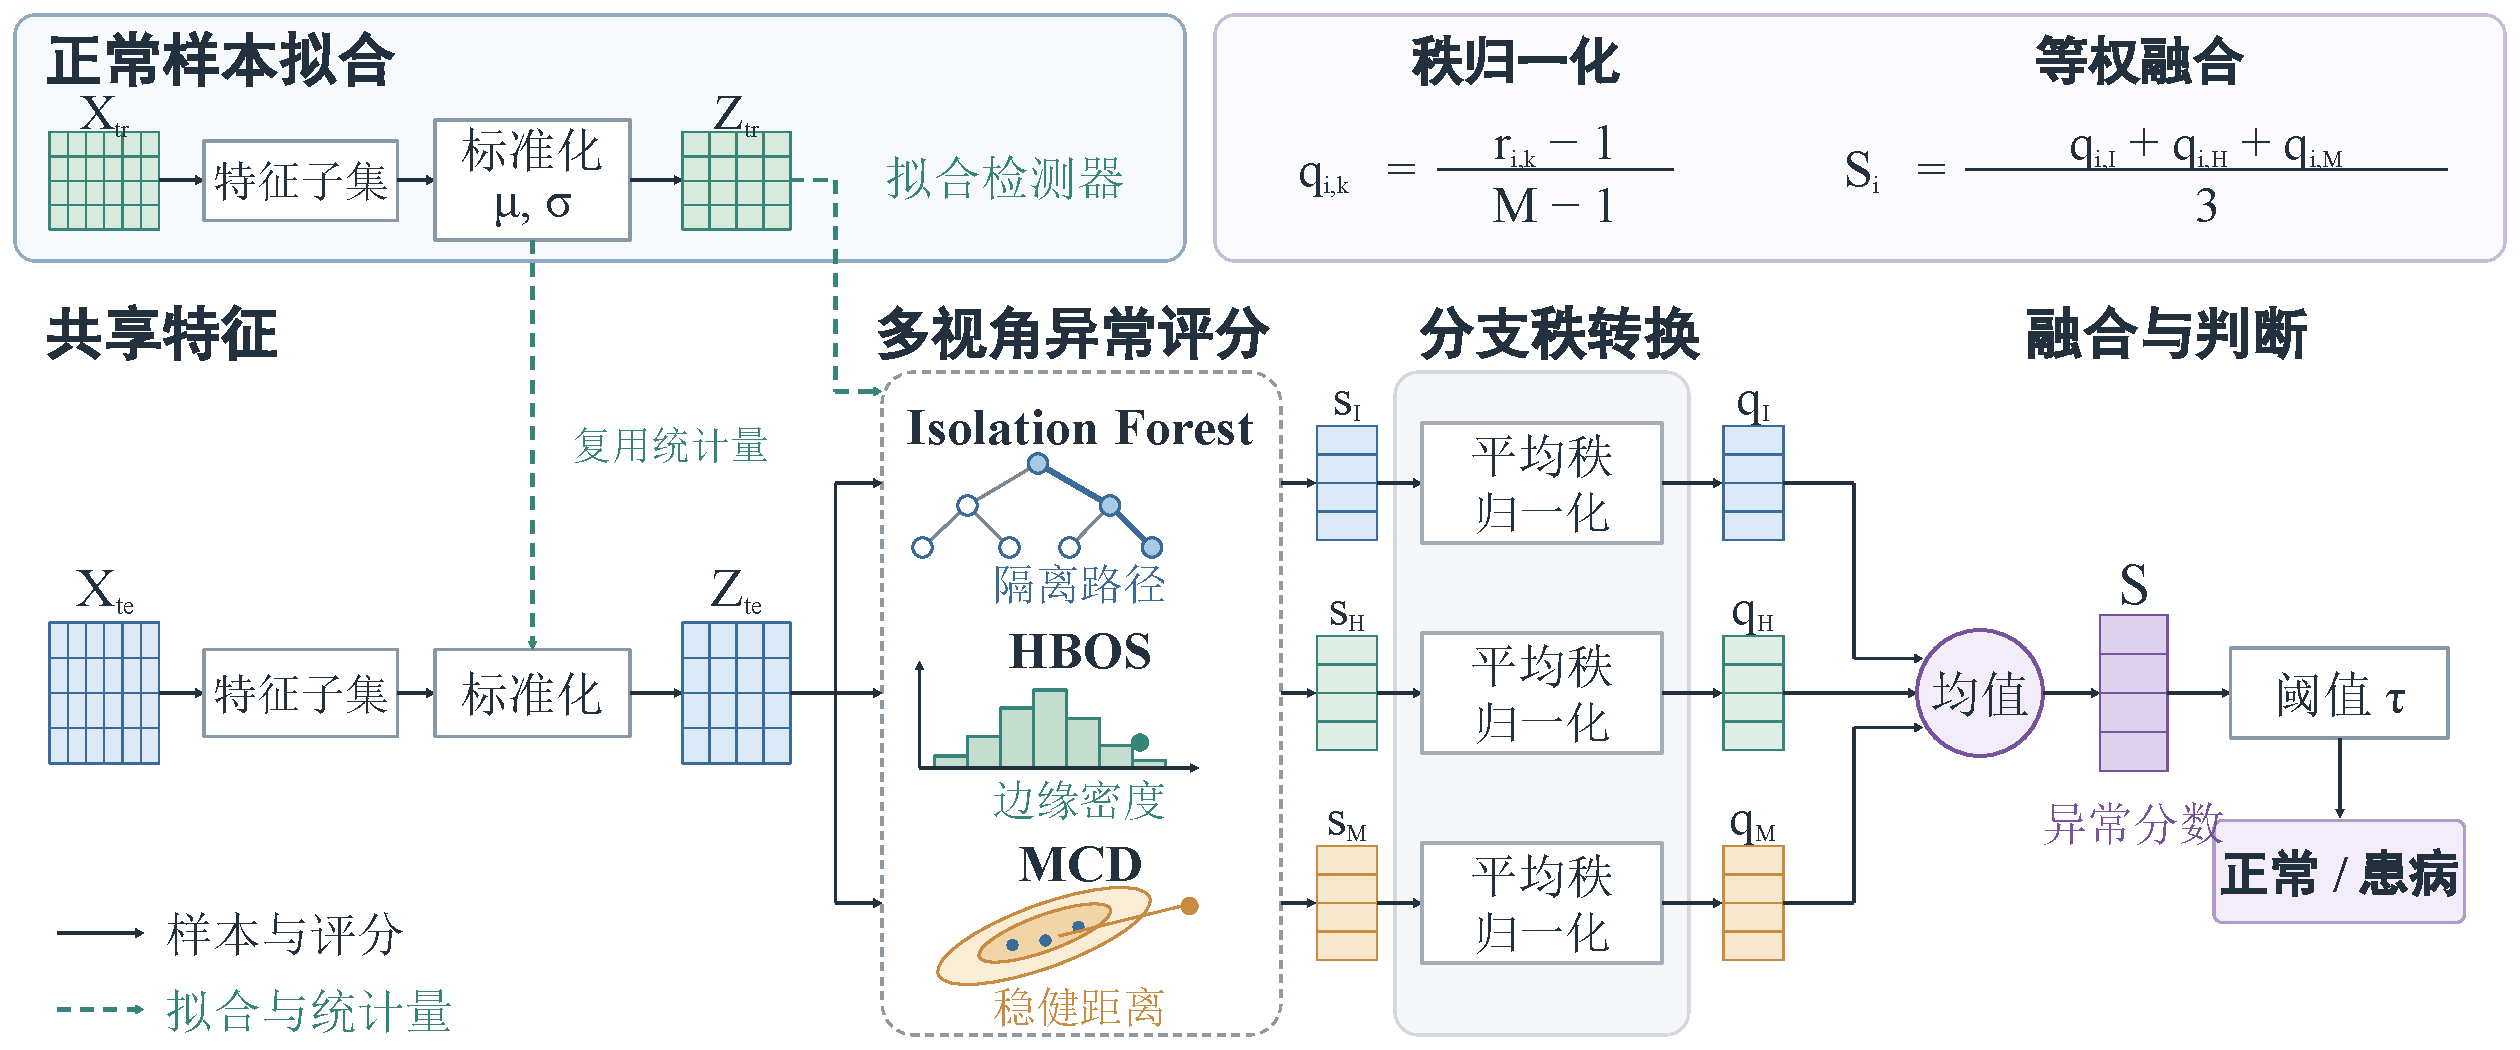
\includegraphics[width=\textwidth]{figures/method-overview.pdf}
  \Description{上方正常样本估计标准化统计量并拟合三个检测器，下方待测样本复用统计量，经过 Isolation Forest、HBOS 和 MCD 三个分支评分、平均秩归一化及等权平均后，依据阈值判断为正常或患病。绿色虚线表示拟合及统计量传递，实线表示样本与评分流。}
  \caption{多检测器秩融合的甲状腺疾病判断框架}
  \label{fig:task4-framework}
\end{figure*}

\subsection{任务定义}
设正常样本集合为
\begin{equation}
  \mathcal D_{\mathrm{tr}}=\{\vect x_i\}_{i=1}^{N},
  \qquad \vect x_i\in\mathbb R^{D},
  \label{eq:task4-train}
\end{equation}
其中 $D$ 为原始特征维度。待测批次记为 $\mathcal B=\{\vect x'_i\}_{i=1}^{M}$，对应的评价标签为 $y_i\in\{0,1\}$，其中 $0$ 表示正常，$1$ 表示患病。模型学习正常样本的统计特征，为每个待测样本给出异常分数 $S_i$。较大的分数表示该样本更偏离正常模式。给定阈值 $\tau$，二元判断为
\begin{equation}
  \widehat y_i(\tau)=\mathbb I(S_i\geq\tau),
  \label{eq:task4-prediction}
\end{equation}
其中 $\mathbb I(\cdot)$ 为指示函数。

\subsection{共享特征与标准化}
设选定的特征索引集合为 $\mathcal J$，通过投影 $P_{\mathcal J}$ 得到 $d=|\mathcal J|$ 维输入向量 $\vect u=P_{\mathcal J}\vect x$。

对正常样本中第 $j$ 个选定特征计算均值与标准差
\begin{equation}
\begin{aligned}
  \mu_j&=\frac{1}{N}\sum_{i=1}^{N}u_{i,j},\\
  \sigma_j&=\sqrt{\frac{1}{N}\sum_{i=1}^{N}(u_{i,j}-\mu_j)^2}.
\end{aligned}
\label{eq:task4-statistics}
\end{equation}
样本的标准化表示为
\begin{equation}
  z_j=\frac{u_j-\mu_j}{\sigma_j},
  \qquad \vect z\in\mathbb R^d.
  \label{eq:task4-standardization}
\end{equation}
该变换将各维度表示为相对于正常样本均值的标准差偏移。正常样本与待测样本使用相同的统计量，分别记其标准化表示为 $\vect z_i$ 与 $\vect z'_i$。

\subsection{Isolation Forest 随机隔离分支}
Isolation Forest 通过随机特征和随机切分点递归划分样本，利用隔离路径长度衡量异常程度~\cite{liu2008isolation}。在一棵隔离树的节点内，选取一个特征，并在该特征的取值范围内随机产生切分点，将样本送入左右子节点。偏离密集区域的样本通常能够通过较少的切分被隔离，从而获得较短的路径。

设森林包含 $T$ 棵树，每棵树使用 $\psi$ 个正常样本。样本 $\vect z$ 在第 $t$ 棵树中到达叶节点的深度为 $e_t(\vect z)$，叶节点包含的样本数为 $n_t(\vect z)$。考虑叶节点内尚未完全隔离的样本后，路径长度为
\begin{equation}
  h_t(\vect z)=e_t(\vect z)+c\bigl(n_t(\vect z)\bigr),
  \label{eq:task4-path}
\end{equation}
其中归一化函数采用
\begin{equation}
  c(n)=
  \begin{cases}
    0, & n\leq 1,\\
    1, & n=2,\\
    2\bigl(\ln(n-1)+\gamma\bigr)-\dfrac{2(n-1)}{n}, & n>2,
  \end{cases}
  \label{eq:task4-path-normalizer}
\end{equation}
$\gamma$ 为欧拉常数。根据多棵树的平均路径得到异常分数
\begin{equation}
  s_{\mathrm I}(\vect z)
  =2^{-\frac{1}{T c(\psi)}\sum_{t=1}^{T}h_t(\vect z)}.
  \label{eq:task4-iforest}
\end{equation}
平均路径越短，$s_{\mathrm I}$ 越大，表示样本越容易被随机切分隔离。

\subsection{HBOS 边缘密度分支}
HBOS 对每个特征建立一维直方图，并汇总样本在各维度上的低密度程度~\cite{goldstein2012histogram}。对第 $j$ 维划分 $B$ 个等宽区间，记第 $b$ 个区间为 $I_{j,b}$，宽度为 $\Delta_{j,b}$。落入该区间的正常样本数为
\begin{equation}
  n_{j,b}=\sum_{i=1}^{N}\mathbb I(z_{i,j}\in I_{j,b}).
  \label{eq:task4-bin-count}
\end{equation}
这些频数对应离散区间概率的极大似然估计。设区间概率向量为 $\vect p_j$，其估计目标及闭式解为
\begin{equation}
\begin{aligned}
  \widehat{\vect p}_j
  &=\underset{\substack{p_{j,b}\geq0\\\sum_b p_{j,b}=1}}{\arg\min}
      \left(-\sum_{b=1}^{B}n_{j,b}\log p_{j,b}\right),\\
  \widehat p_{j,b}&=\frac{n_{j,b}}{N}.
\end{aligned}
\label{eq:task4-hist-objective}
\end{equation}
据此得到区间内的概率密度估计
\begin{equation}
  \widehat f_j(v)=\frac{n_{j,b}}{N\Delta_{j,b}},
  \qquad v\in I_{j,b}.
  \label{eq:task4-hist-density}
\end{equation}
以 $\alpha$ 平滑密度后，分支异常分数定义为
\begin{equation}
  s_{\mathrm H}(\vect z)
  =-\sum_{j=1}^{d}\log_2\bigl(\widehat f_j(z_j)+\alpha\bigr).
  \label{eq:task4-hbos}
\end{equation}
低密度区间对异常分数的贡献更大，使单个指标上的偏离能够进入综合评分。直方图范围外的密度按边界规则延拓，具体设置见实验部分。

\subsection{MCD 稳健距离分支}
MCD 通过协方差行列式最小化估计正常样本的中心与散布结构~\cite{rousseeuw1999fast}。设正常样本索引的候选子集为 $\mathcal H$，且 $|\mathcal H|=h$，对应均值与协方差为
\begin{equation}
\begin{aligned}
  \vect\mu_{\mathcal H}
    &=\frac{1}{h}\sum_{i\in\mathcal H}\vect z_i,\\
  \vect\Sigma_{\mathcal H}
    &=\frac{1}{h}\sum_{i\in\mathcal H}
      (\vect z_i-\vect\mu_{\mathcal H})
      (\vect z_i-\vect\mu_{\mathcal H})^{\mathsf T}.
\end{aligned}
\label{eq:task4-mcd-statistics}
\end{equation}
估计目标为
\begin{equation}
  \mathcal H^*
  =\underset{\substack{\mathcal H\subseteq\{1,\ldots,N\}\\|\mathcal H|=h}}{\arg\min}
    \det(\vect\Sigma_{\mathcal H}).
  \label{eq:task4-mcd-objective}
\end{equation}
协方差行列式衡量所选样本的整体散布规模。FAST-MCD 通过候选子集搜索求解这一估计问题，经校正与重加权得到稳健中心 $\widehat{\vect\mu}_{\mathrm R}$ 和协方差 $\widehat{\vect\Sigma}_{\mathrm R}$。

对待测向量，使用平方马氏距离作为异常分数
\begin{equation}
  s_{\mathrm M}(\vect z)
  =(\vect z-\widehat{\vect\mu}_{\mathrm R})^{\mathsf T}
   \widehat{\vect\Sigma}_{\mathrm R}^{\dagger}
   (\vect z-\widehat{\vect\mu}_{\mathrm R}),
  \label{eq:task4-mcd-score}
\end{equation}
其中 $\dagger$ 表示矩阵伪逆。协方差将特征之间的相关关系纳入距离计算，刻画样本相对于正常中心的联合偏离。

\subsection{平均秩归一化与等权融合}
三个分支的分数尺度不同，融合时使用样本在各分支中的相对异常次序。记检测器索引集合为 $\mathcal K=\{\mathrm I,\mathrm H,\mathrm M\}$，分支数为 $K=|\mathcal K|$。对同一待测批次，分支评分 $s_{i,k}=s_k(\vect z'_i)$ 的升序平均秩为
\begin{equation}
  r_{i,k}=\operatorname{rank}_{\mathrm{avg}}
     \bigl(s_{i,k}\,;\,s_{1,k},\ldots,s_{M,k}\bigr).
  \label{eq:task4-rank}
\end{equation}
分数相同的样本使用其占据名次的平均值，秩的起点为 $1$。将平均秩转换为
\begin{equation}
  q_{i,k}=\frac{r_{i,k}-1}{M-1},
  \qquad q_{i,k}\in[0,1].
  \label{eq:task4-rank-normalization}
\end{equation}
该映射保留各分支的排序信息，并将其置于统一的数值范围内。对 $K$ 个检测器等权平均，得到
\begin{equation}
  S_i=\frac{1}{K}\sum_{k\in\mathcal K}q_{i,k}.
  \label{eq:task4-fusion}
\end{equation}
样本在多个分支中获得较高异常名次时，融合分数相应增大。$S_i$ 表示样本在该待测批次内的相对异常程度，代入式~\eqref{eq:task4-prediction} 得到二元判断。
